\documentclass[12pt,a4paper]{article}
\usepackage[utf8]{inputenc} % inutile avec XeLaTeX/LuaLaTeX
\usepackage[T1]{fontenc}
\usepackage{amsmath,amssymb,mathrsfs,tikz,times,pifont}
\usepackage{enumitem}
\usepackage{multicol}
\usepackage{lmodern}
\newcommand\circitem[1]{%
\tikz[baseline=(char.base)]{
\node[circle,draw=gray, fill=red!55,
minimum size=1.2em,inner sep=0] (char) {#1};}}
\newcommand\boxitem[1]{%
\tikz[baseline=(char.base)]{
\node[fill=cyan,
minimum size=1.2em,inner sep=0] (char) {#1};}}
\setlist[enumerate,1]{label=\protect\circitem{\arabic*}}
\setlist[enumerate,2]{label=\protect\boxitem{\alph*}}
\everymath{\displaystyle}
\usepackage[left=1cm,right=1cm,top=1cm,bottom=1.7cm]{geometry}
\usepackage[colorlinks=true, linkcolor=blue, urlcolor=blue, citecolor=blue]{hyperref}
\usepackage{array,multirow}
\usepackage[most]{tcolorbox}
\usepackage{varwidth}
\usepackage{float}
\tcbuselibrary{skins,hooks}
\usetikzlibrary{patterns}

\newtcolorbox{exa}[2][]{enhanced,breakable,before skip=2mm,after skip=5mm,
colback=yellow!20!white,colframe=black!20!blue,boxrule=0.5mm,
attach boxed title to top left ={xshift=0.6cm,yshift*=1mm-\tcboxedtitleheight},
fonttitle=\bfseries,
title={#2},#1,
boxed title style={frame code={
\path[fill=tcbcolback!30!black]
([yshift=-1mm,xshift=-1mm]frame.north west)
arc[start angle=0,end angle=180,radius=1mm]
([yshift=-1mm,xshift=1mm]frame.north east)
arc[start angle=180,end angle=0,radius=1mm];
\path[left color=tcbcolback!60!black,right color = tcbcolback!60!black,
middle color = tcbcolback!80!black]
([xshift=-2mm]frame.north west) -- ([xshift=2mm]frame.north east)
[rounded corners=1mm]-- ([xshift=1mm,yshift=-1mm]frame.north east)
-- (frame.south east) -- (frame.south west)
-- ([xshift=-1mm,yshift=-1mm]frame.north west)
[sharp corners]-- cycle;
},interior engine=empty,
},interior style={top color=yellow!5}}

\usepackage{fancyhdr}
\usepackage{eso-pic}
\usepackage{tkz-tab}
\AddToShipoutPicture{
    \AtTextCenter{%
        \makebox[0pt]{\rotatebox{80}{\textcolor[gray]{0.7}{\fontsize{5cm}{5cm}\selectfont PGB}}}
    }
}

\usepackage{verbatim}

\usepackage{color,soul}

\usepackage{amsmath}
\usepackage{amsfonts}
\usepackage{amssymb}
\usepackage{systeme}
\usepackage{tkz-tab}
\usepackage{tikz}
\usetikzlibrary{arrows}
\newcounter{exemple} % Compteur pour les questions

% Définir la commande pour afficher une question numérotée
\newcommand{\exemple}{%
  \refstepcounter{exemple}%
  \textbf{\textcolor{green}{Exemple \theexemple :}} \ignorespaces
}
%---------------------------------------
\definecolor{myorange}{rgb}{1.0, 0.8, 0.0}

% Définir un compteur pour les exercices d'application
\newcounter{exerciceapp}

% Définir la commande pour afficher un exercice d'application numéroté
\newcommand{\exerciceapp}{%
  \refstepcounter{exerciceapp}%
  \textbf{\textcolor{myorange}{Exercice d'application \theexerciceapp :}} \ignorespaces
}
%--------------------------------------
% Définir un compteur pour les exercices d'application
\newcounter{correction}

% Définir la commande pour afficher un correction exercice d'application numéroté
\newcommand{\correction}{%
  \refstepcounter{correction}%
  \textbf{\textcolor{myorange}{Correction \thecorrection :}} \ignorespaces
}
%--------------------------------------
% Commande pour ajouter du texte en arrière-plan
\usepackage{fancyhdr}
\usepackage{eso-pic}
%\usepackage{tkz-tab}
\AddToShipoutPicture{
    \AtTextCenter{%
        \makebox[0pt]{\rotatebox{80}{\textcolor[gray]{0.7}{\fontsize{5cm}{5cm}\selectfont PGB}}}
    }
}
%This command takes a colour as an optional argument; the default colour is black.
\usetikzlibrary{shapes.geometric,fit}
\newcommand{\myul}[2][black]{\setulcolor{#1}\ul{#2}\setulcolor{black}}
\newcommand\tab[1][1cm]{\hspace*{#1}}

\begin{document}
% En-tête personnalisée
\begin{center}
    \Large\textbf{\underline{Nombres Complexes}}\\[-0.1cm]
    \normalsize\textbf{Prof : M. BA} \hfill \textbf{Classe : TS2}\\[-0.1cm]
    \textbf{Année scolaire : 2024 -- 2025}
\end{center}

\section*{Introduction aux Nombres Complexes}

Les nombres complexes, que nous allons explorer dans ce cours, ont une origine intrigante liée à la résolution des équations polynomiales. Au cours de l'histoire des mathématiques, des énigmes telles que la résolution de l'équation cubique $x^3 + ax^2 + bx + c = 0$ ont captivé l'attention des mathématiciens.

Au XVIe siècle, l'équation cubique a été résolue par le mathématicien italien Niccolò Fontana, également connu sous le nom de Tartaglia. Cependant, il est intéressant de noter que la tentative de résolution de certaines équations cubiques conduisit à l'introduction des nombres complexes.

L'équation $x^2 + 1 = 0$, apparemment insoluble dans l'ensemble des nombres réels, était une pierre d'achoppement dans la résolution des équations cubiques. Pourtant, pour surmonter cette difficulté, les mathématiciens du XVIe siècle, tels que Gerolamo Cardano et Rafael Bombelli, ont introduit une unité imaginaire, notée $i$, qui était la solution de l'équation $i^2 = -1$. Cette innovation a été la première étape vers la création de l'ensemble des nombres complexes.

Ainsi, les nombres complexes ne sont pas seulement une extension abstraite des nombres réels, mais ils ont émergé de la nécessité de résoudre des problèmes concrets en algèbre. Dans ce cours, nous explorerons les propriétés fascinantes et les applications puissantes des nombres complexes.

Préparez-vous à plonger dans le monde fascinant des nombres complexes, où l'imagination des mathématiciens a transcendé les limites des nombres réels pour créer un outil puissant et élégant.

\section*{\underline{\textbf{\textcolor{red}{I.Définition et notations }}}}

On appelle ensemble des nombres complexes l'ensemble noté $\mathbb{C}$ qui :

\begin{itemize}
  \item[$\blacktriangleright$] contient l'ensemble des réels $\mathbb{R}$ : $\mathbb{R} \subset \mathbb{C}$
  \item[$\blacktriangleright$] est muni de l'addition et de la multiplication, possédant les mêmes propriétés que $\mathbb{R}$ (commutativité, associativité, élément neutre, élément symétrique ou opposé, distributivité, etc.)
  \item[$\blacktriangleright$] contient un élément noté $i$ vérifiant $i^{2}=-1$
\end{itemize}

$\bullet$ Tout nombre complexe $z \in \mathbb{C}$ s'écrit, de façon algébrique, sous la forme $z=a+ib$, où $a$ et $b$ sont des nombres réels. 

$a$ est appelé la partie réelle de $z$ notée $\mathcal{R}e(z)=a$, et $b$ est appelé la partie imaginaire de $z$ notée $\mathcal{I}m(z)=b$.

$\bullet$ Le nombre complexe $z=a+ib$ est réel si, et seulement si, $b=0$ (c'est-à-dire $\mathcal{I}m(z)=0$).

$\bullet$ Le nombre complexe $z=a+ib$ est imaginaire pur si, et seulement si, $a=0$ (c'est-à-dire $\mathcal{R}e(z)=0$).

$\bullet$ Le nombre complexe $z=a+ib$ est nul si, et seulement si,
\[
  \systeme{a=0, b=0}
  \iff
  \systeme{\mathcal{R}e(z)=0, \mathcal{I}m(z)=0}
\]

$\bullet$ Soient $z$ et $z'$ deux nombres complexes tels que $z=a+ib$ et $z'=a'+ib'$, alors $z=z'$ si, et seulement si,
\[
  \systeme{a=a', b=b'}
  \iff
  \systeme{\mathcal{R}e(z)=\mathcal{R}e(z'), \mathcal{I}m(z)=\mathcal{I}m(z')}
\]

\underline{\exemple}\\
Soit le nombre complexe \(z = 3 - 4i\).

\begin{itemize}
  \item[$\bullet$] La partie réelle de \(z\) est \(\mathcal{R}e(z) = 3\).
  \item[$\bullet$] La partie imaginaire de \(z\) est \(\mathcal{I}m(z) = -4\).
  \item[$\bullet$] \(z\) n'est pas un réel car \(\mathcal{I}m(z) \neq 0\).
  \item[$\bullet$] \(z\) n'est pas imaginaire pur car \(\mathcal{R}e(z) \neq 0\).
  \item[$\bullet$] Le conjugué de \(z\) est \(\overline{z} = 3 + 4i\).
\end{itemize}

\underline{\textbf{\textcolor{red}{Remarque }}}\\
Dans $\mathbb{C}$, où $a$ et $b$ sont des nombres réels. Les identités remarquables deviennent:
\[
  \begin{aligned}
    (a+ib)^{2} &= a^{2}+2iab-b^{2}, \\
    (a-ib)^{2} &= a^{2}-2iab-b^{2}.
  \end{aligned}
\]

\underline{\exemple}\\
Considérons le nombre complexe $z=2+3i$. Appliquons les identités remarquables :
\[
  \begin{aligned}
    (2+3i)^{2} &= (2)^{2} + 2 \cdot 2 \cdot 3i + (3i)^{2} \\
               &= 4 + 12i - 9 \\
               &= -5 + 12i.
  \end{aligned}
\]


De même, pour $z$, $\overline{z} = 2-3i$, appliquons l'identité remarquable correspondante :
\[
  \begin{aligned}
    (2-3i)^{2} &= (2)^{2} - 2 \cdot 2 \cdot 3i + (3i)^{2} \\
               &= 4 - 12i - 9 \\
               &= -5 - 12i.
  \end{aligned}
\]

\section*{\underline{\textbf{\textcolor{red}{II. Conjugué d'un Nombre Complexe }}}}

\underline{\textbf{\textcolor{red}{1.Définition}}}

Soit $z = a + ib$ un nombre complexe, où $a$ et $b$ sont des nombres réels, le conjugué de $z$, noté $\overline{z}$, est obtenu en changeant le signe de la partie imaginaire, c'est-à-dire $\overline{z} = a - ib$.

\underline{\exemple}

Le conjugué de $w = 3 + 2i$ est $\overline{w}=3-2i$

\underline{\textbf{\textcolor{red}{2.Propriétés}}}\
\begin{itemize}
\item[$\bullet$] Le conjugué du conjugué : $\overline{\overline{z}} = z$.
\item[$\bullet$] La somme des conjugués est égale à la conjugaison d'une somme : $\overline{z_1 + z_2} = \overline{z_1} + \overline{z_2}$.
\item[$\bullet$] Le conjugué du produit est égal au produit des conjugués : $\overline{z_1 \cdot z_2} = \overline{z_1} \cdot \overline{z_2}$.
\item[$\bullet$] Le conjugué d'un quotient est égal au quotient des conjugués : $\overline{\left(\frac{z_1}{z_2}\right)} = \frac{\overline{z_1}}{\overline{z_2}}$, pour $z_2 \neq 0$.
\item[$\bullet$] $p\in\mathbb{Z}$ $\overline{z^{p}} = \overline{z}^{p}$ 
\item[$\bullet$] $z$ est réel si, et seulement si, $ \overline{z} = z $.
\item[$\bullet$] $z$ est imaginaire pur si, et seulement si, $\overline{z} = -z$.
\item[$\bullet$] $\mathcal{R}e(z)=\frac{z+\overline{z}}{2}$
\item[$\bullet$] $\mathcal{I}m(z)=\frac{z-\overline{z}}{2i}$
\end{itemize}

\underline{\exemple}

\begin{enumerate}
\item Considérons deux nombres complexes $z_1 = 2 + 3i$ et $z_2 = 1 - 2i$. 

Calculons les conjugués et vérifions les propriétés :

\begin{itemize}
\item[$\bullet$] Le conjugué du conjugué : $\overline{\overline{z_1}} = \overline{\overline{2 + 3i}} = 2 + 3i = z_1$.
\item[$\bullet$] La somme des conjugués : $\overline{z_1 + z_2} = \overline{3 + i} = 3 - i = \overline{z_1} + \overline{z_2}$.
\item[$\bullet$] Le produit des conjugués : $\overline{z_1 \cdot z_2} = \overline{8 + 5i} = 8 - 5i = \overline{z_1} \cdot \overline{z_2}$.
\item[$\bullet$] Le conjugué du produit : $\overline{z_1 \cdot z_2} = \overline{-4 - 7i} = -4 + 7i = \overline{z_1} \cdot \overline{z_2}$.
\item[$\bullet$] Le conjugué d'un rapport : $\overline{(\frac{z_1}{z_2})} = \frac{\overline{2 + 3i}}{\overline{1 - 2i}} = \frac{2 - 3i}{1 + 2i}$.

\end{itemize}
\item Soit \(z = 1 + i\) et \(p = 3\). 

Vérifions que  \(\overline{z^3} = \overline{z}^3 \)

On a :
\(
z^3 = (1 + i)^3 = -2 + 2i.
\)

Donc :
\(
\overline{z^3} = \overline{-2 + 2i} = -2 - 2i.
\)

D'autre part :
\(
\overline{z} = 1 - i, \quad \overline{z}^3 = (1 - i)^3 = (1 - i)(1 - i)(1 - i) = -2 - 2i.
\)

Ainsi, \(\overline{z^3} = \overline{z}^3\).
\end{enumerate}

\section*{\underline{\textbf{\textcolor{red}{III. Représentation graphique d'un Nombre Complexe }}}}

Les nombres complexes peuvent être vus comme des points du plan appelé.

Chaque nombre complexe est représenté par un point unique dans ce plan, où l'axe horizontal correspond à la partie réelle et l'axe vertical à la partie imaginaire.

\underline{\textbf{\textcolor{red}{1.Plan Complexes}}}

Le plan complexe est un plan muni d'un repère cartésien. 

Chaque nombre complexe $z = a + ib$ peut être associé à un point $(a, b)$ dans ce plan.

Le nombre complexe $z = a + i b$ est appelé l'affixe du point $M$. 

On peut donc noter sans ambiguïté $M(z)$ le point $M$ d'affixe $z$.

$z$ est l'affixe de $M$

$M$ est l'image de $z$

On note $M(z)$
\begin{tikzpicture}[scale=1.5]
  % Axes
  \draw[->] (-2,0) -- (2,0) node[right] {$\Re$};
  \draw[->] (0,-2) -- (0,2) node[above] {$\Im$};
  
  % Points
  \fill (1,1) circle[radius=2pt] node[above right] {$z = a + bi$};
  
  % Lignes auxiliaires
  \draw[dashed] (1,0) -- (1,1) node[midway, right] {$b$};
  \draw[dashed] (0,1) -- (1,1) node[midway, above] {$a$};
\end{tikzpicture}
\begin{tikzpicture}[scale=2]
  % Axes
  \draw[->] (-2,0) -- (2,0) node[right] {$\Re$};
  \draw[->] (0,-2) -- (0,2) node[above] {$\Im$};
  
  % Repère gradué
  \foreach \x in {-2,-1.5,...,2}
    \draw (\x,-0.05) -- (\x,0.05) node[below=2pt] {\tiny $\x$};
  \foreach \y in {-2,-1.5,...,2}
    \draw (-0.05,\y) -- (0.05,\y) node[left=2pt] {\tiny $\y$};
  
  % Points
  \fill (1,1) circle[radius=2pt] node[above right] {$z = a + bi$};
  
  % Lignes auxiliaires
  \draw[dashed] (1,0) -- (1,1) node[midway, right] {$b$};
  \draw[dashed] (0,1) -- (1,1) node[midway, above] {$a$};
\end{tikzpicture}
\\
\begin{tikzpicture}[scale=2]
  % Axes
  \draw[->] (-2,0) -- (2,0) node[right] {$\Re$};
  \draw[->] (0,-2) -- (0,2) node[above] {$\Im$};
  
  % Repère gradué
  \foreach \x in {-2,-1.5,...,2}
    \draw (\x,-0.05) -- (\x,0.05) node[below=2pt] {\tiny $\x$};
  \foreach \y in {-2,-1.5,...,2}
    \draw (-0.05,\y) -- (0.05,\y) node[left=2pt] {\tiny $\y i$};
  
  % Points
  \fill (1,1) circle[radius=2pt] node[above right] {$z = a + bi$};
  
  % Lignes auxiliaires
  \draw[dashed] (1,0) -- (1,1) node[midway, right] {$b$};
  \draw[dashed] (0,1) -- (1,1) node[midway, above] {$a$};
\end{tikzpicture}
\\	
\textbf{\textcolor{yellow}{Cette équivalence permet de considérer le plan orienté muni d'un repère orthonormé direct comme une « représentation » de l'ensemble des nombres complexes}}

\underline{\textbf{\textcolor{red}{2.Représentation d'un Nombre Complexe}}}

Soit $z = a + ib$ un nombre complexe. Le point associé dans le plan complexe est $(a, b)$.\\
\textbf{\textcolor{yellow}{On peut également utiliser la forme polaire pour représenter un nombre complexe en utilisant sa distance au point d'origine et l'angle qu'il forme avec l'axe des abscisses}}.

\underline{\exemple}

Considérons le nombre complexe $z = 3 + 4i$. 

Le point associé dans le plan complexe est $(3, 4)$.\\
Représenter $z$ et $\overline{z}$\\

\begin{tikzpicture}[>=stealth]
    % Axes
    \draw[->] (-1, 0) -- (4, 0) node[below] {\quad Re};
    \draw[->] (0, -1) -- (0, 4) node[left] {Im};
    % Point z
    \draw[->, thick, blue] (0, 0) -- (3, 2) node[midway, above left] {$z$};
    \fill (3, 2) circle (2pt) node[above right] {$(3, 2)$};
    % Grille
    \draw[dashed, gray] (3, 0) -- (3, 2) -- (0, 2);
    \node[below] at (3, 0) {3};
    \node[left] at (0, 2) {2};
\end{tikzpicture}

\section*{\underline{\textbf{\textcolor{red}{IV. Module d'un Nombre Complexe}}}}
\subsection*{\underline{\textbf{\textcolor{red}{1.Définition  }}}} 
Le module de $z$, noté $|z|$, est défini comme la distance entre le point représentant $z$ et l'origine $(0,0)$ dans le plan complexe.

Le module d'un nombre complexe $z = a + ib$ est défini comme :
\[ |z| = \sqrt{a^2 + b^2} \]

\subsection*{\underline{\textbf{\textcolor{red}{2.Propriétés}}}}

Le module d'un nombre complexe possède plusieurs propriétés importantes :

\begin{itemize}
\item[$\bullet$] Le module d'un conjugué : $|\overline{z}| = |z|$.
\item[$\bullet$] Le module d'un produit : $|z_1 \cdot z_2| = |z_1| \cdot |z_2|$.
\item[$\bullet$] Le module d'une puissance : $|z^n| = |z|^n$.
\item[$\bullet$] Le module d'un conjugué : $z\overline{z} = |z|=\sqrt{a^2 + b^2}$.
\item[$\bullet$] Inégalité triangulaire : Pour tous \(z_1, z_2 \in \mathbb{C}\),\(|z_1 + z_2| \leq |z_1| + |z_2|\)
\item[$\bullet$] Pour deux points \(A\) et \(B\) d’affixes respectives \(z_A\) et \(z_B\), la distance \(AB\) entre ces points est donnée par : $|z_A - z_B| =AB$.
\end{itemize}

\underline{\exemple}

Soit $z = 3 + 4i$. Calculons son module $|z|$.puis $|z^{5}|$.

\[ |z| = \sqrt{3^2 + 4^2} = \sqrt{9 + 16} = \sqrt{25} = 5 \]

Le module de $z$ est donc $5$.\\
\[ |z^{5}| =|z|^{5}=(\sqrt{3^2 + 4^2})^{5} = (\sqrt{9 + 16})^{5} = (\sqrt{25})^{5} = (\sqrt{5})^{4+1} = 25\sqrt{5} \]
%Les propriétés du module sont essentielles dans de nombreux calculs et démonstrations impliquant des nombres complexes. Elles fournissent une mesure de la taille d'un nombre complexe dans le plan complexe.\\

\underline{\textbf{\textcolor{green}{Exerice 1.a 1.b 1.c 1.d CIAM SE PAGE 2010}}}

\underline{\textbf{\textcolor{green}{Exerice 1.e 1.f 1.g CIAM SE PAGE 2012}}}

\textbf{\exerciceapp}

$z_{1}=-\sqrt{3}+i$ ; $z_{2}=2(-\sqrt{3}+i)$ ; $z_{3}=(-\sqrt{3}+i)(1+i)^{2}$ ; 
$z_{4}=\frac{(-\sqrt{3}+i)^{3}}{(1+i)^{2}}$ ; $z_{4}=\frac{(1+i)^{3}}{3+2i}$

1.Calcule le module de ces nombres complexe

2.Le plan est muni d'un repère orthonormal $(O,\vec{u},\vec{v})$.

Soit A, B et C les affixes respectives $1-3i$ ; $4+5i$ ; $-3+2i$.

Calculer: AB ; AC ; BC.

\section*{\underline{\textbf{\textcolor{red}{V. Argument d'un nombre complexe non nul }}}}
\subsection*{\underline{\textbf{\textcolor{red}{1.Définition}}}}
Soit z un nombre complexe non nul sur le repère othonormal $(O,\vec{u},\vec{v})$. L'argument du nombre complexe $z = a + ib$ non nul est l'angle en radian que le vecteur correspondant à $z$ forme avec l'axe des abscisses dans le plan complexe.\\ On note généralement $arg(z)=mes(\widehat{\vec{u},\vec{OM}})$\\
En notant $\theta$ on a : $\cos(\theta)=\frac{\mathcal{R}e(z)}{|z|}$ et 
$\sin(\theta)=\frac{\mathcal{I}m(z)}{|z|}$\\
\underline{\textbf{\textcolor{red}{Rappelle}}}\\
Tableau trigonométrique\\
Cercles trigonométrie\\
\subsection*{\underline{\textbf{\textcolor{red}{2.Propiétés}}}}
Soit z et z' deux nombrs complexes ,et $n\in \mathbb{N}$\\
\begin{itemize}
\item[$\bullet$] $\text{{arg}}(z_1 \cdot z_2) = \text{{arg}}(z_1) + \text{{arg}}(z_2)[2\pi]$\\
\item[$\bullet$] $\text{{arg}}(\frac{z_1}{z_2}) = \text{{arg}}(z_1) - \text{{arg}}(z_2)[2\pi]$\\
\item[$\bullet$] $\text{{arg}}(\frac{1}{z_2}) = - \text{{arg}}(z_2)[2\pi]$\\
\item[$\bullet$] $\text{{arg}}((z_2)^{n}) = n\text{{arg}}(z_2)[2\pi]$\\
\item[$\bullet$] $\text{{arg}}(-z_2) = \text{{arg}}(z_2)+\pi[2\pi]$\\
\item[$\bullet$] $\text{{arg}}(\overline{z}) = -\text{{arg}}(z)[2\pi]$\\
\item[$\bullet$] soit $z_A$ ; $z_B$ ; $z_C$ les affixes respectives des points A, B et C les image de ces complexes dans le repère orthonormal $(O,\vec{u},\vec{v})$. tel que $z_A \neq z_B$ ; 
$z_C \neq z_A$ $arg(z_A-z_B)=(\vec{u},\overrightarrow{AB})$
\item[$\bullet$] $arg(\frac{z_C-z_A}{z_B-z_A})=(\widehat{\overrightarrow{AB},\overrightarrow{AC}})$
\end{itemize}

\textbf{\exerciceapp}

Déterminer l'argument des nombres complexes suivnats\\
$z_{1}=-\sqrt{3}+i$ ; $z_{2}=2(-\sqrt{3}+i)$ ; $z_{3}=(-\sqrt{3}+i)(1+i)^{2}$ ; 
$z_{4}=\frac{(-\sqrt{3}+i)^{3}}{(1+i)^{2}}$ ; $z_{4}=\frac{(1+i)^{3}}{3+2i}$\\
\textbf{\correction}\\
\underline{\textbf{\textcolor{red}{Remarque}}}\\
\begin{itemize}
\item[$\bullet$]Si $arg(z)=0$ alors z est un réel positif
\item[$\bullet$]Si z est une réel négatif alors $arg(z)=\pi$
\item[$\bullet$]Si $z=ib$ (imaginaire pur) alors :\\
Si $b>0$ alors $arg(z)=\frac{\pi}{2}$\\
Si $b<0$ alors $arg(z)=\frac{-\pi}{2}$
\end{itemize}

\section*{\underline{\textbf{\textcolor{red}{VI. Forme d'un nombre complexe }}}}
\subsection*{\underline{\textbf{\textcolor{red}{1. Forme algébrique d'un nombre Complexe}}}}
Soit $a$ et $b$ des réels, l'écriture $z=a+ib$ est appélé forme algébrique du nombre complexe.

\underline{\exemple}\\
Donner la forme algébrique dans chaque cas
\subsection*{\underline{\textbf{\textcolor{red}{2. Forme trigonométrique d'un nombre Complexe}}}}
Soit z un nombre complexe non nul d'argument $\theta$. On appelle forme trigonométrique d'un nombre complexe l'écriture suivante:\\
$z=|z|(cos(\theta)+isin(\theta))$\\
Avec $cos(\theta)=\frac{\Re(z)}{|z|}$ et $sin(\theta)=\frac{\Im(z)}{|z|}$\\
\underline{\exemple}\\
Donner la forme trigonométrique des nombres complexes suivantes:\\
$z_{1}=1+i\sqrt{3}$ ; $z_{2}=-\sqrt{3}+3i$ ; $z_{3}=\frac{-\sqrt{2}}{1-i}$\\
\underline{\textbf{\textcolor{red}{Solution}}}\\
\subsection*{\underline{\textbf{\textcolor{red}{3. Forme exponentielle d'un nombre complexe non nul}}}}
\subsection*{\underline{\textbf{\textcolor{blue}{a. Définition }}}}
On pose $cos(\theta)+isin(\theta)=e^{i\theta}$\\
Soit z un nombre complexe non nul d'argument $\theta$ i.e $\arg(z)=\theta$.
 
On appelle forme exponentielle d'un nombre complexe l'écriture : $z=|z|e^{i\theta}$
\subsection*{\underline{\textbf{\textcolor{blue}{b. Propriétés }}}}
Soit $z_{1}=e^{i\theta_{1}}$ et $z_{2}=e^{i\theta_{1}}$ on a:\\
$z=e^{i\theta_{1}} \times e^{i\theta_{2}} = e^{i(\theta_{1}+\theta_{2})}$\\
$z=\frac{e^{i\theta_{1}}}{e^{i\theta_{2}}} = e^{i(\theta_{1}-\theta_{2})}$\\
$z=\frac{1}{e^{i\theta}} = e^{-i\theta}$\\
$z^{n}=(e^{i\theta_{1}})^{n}=e^{in\theta_{1}}$\\
\textbf{\exerciceapp}\\
Donne la forme exponentielle des nombres complexes suivants:\\
$z_{1}=-\sqrt{3}+i$ ; $z_{2}=-\sqrt{6}+i\sqrt{2}$ et $z_{3}=1+i\sqrt{3}$\\
\textbf{\correction}\\
\section*{\underline{\textbf{\textcolor{red}{VII.Formule de Moivre-Formule d'Euler }}}}
\subsection*{\underline{\textbf{\textcolor{red}{1.Formule de Moivre }}}}
A partir de la forme trigonométrique d'un nombre complexe on peut déduire la formule de Moivre.\\
$\forall \theta \in \mathbb{R}$ et $n \in \mathbb{Z}$,\\
$(cos(\theta)+isin(\theta))^{n}=cos(n\theta)+isin(n\theta)$\\
$(cos(\theta)-isin(\theta))^{n}=cos(n\theta)-isin(n\theta)$\\

\subsection*{\underline{\textbf{\textcolor{red}{2.Formule d'Euler}}}}
A partir de la forme exponentielle d'un nombre complexe on peut déduire les formules\\ d'Euler.\\
$cos(\theta)\frac{e^{i\theta}+e^{-i\theta}}{2}$ $sin(\theta)\frac{e^{i\theta}-e^{-i\theta}}{2i}$\\
$cos(n\theta)=\frac{e^{ni\theta}+e^{-ni\theta}}{2} $ $sin(n\theta)=\frac{e^{ni\theta}-e^{-ni\theta}}{2i}$\\
\subsection*{\underline{\textbf{\textcolor{red}{3.Linéariser des expressions trigonométriques:}}}}

\underline{\exemple}\\
Linéariser $sin^{3}(x)$ et $cos^{3}(x)$\\
\underline{\textbf{\textcolor{red}{Solution}}}\\
$cos^{3}(x)=\frac{1}{4}cos(3x)+\frac{3}{4}cos(x)$\\
$sin^{3}(x)=\frac{-1}{4}sin(3x)+\frac{3}{4}sin(x)$
\section*{\underline{\textbf{\textcolor{red}{VIII.Résolution d'équations dans $\mathbb{C}$}}}}
\subsection*{\underline{\textbf{\textcolor{red}{1.Déterminer les racines nièmes $(n\geq2)$ d'un complexe:}}}}
\underline{\textbf{\textcolor{blue}{a. Racine n-ième de l’unité}}}

Les \textbf{racines n-ièmes de l’unité} sont les solutions complexes de l’équation suivante :
\[
z^n = 1,
\]
où \(n \in \mathbb{N}^*\) est un entier naturel non nul.

Elles sont appelées ainsi car leur module est toujours égal à \(1\), ce qui signifie qu’elles appartiennent au cercle unité dans le plan complexe.

\paragraph{\underline{\textbf{\textcolor{blue}{Formule générale :}}}}

Les \(n\) racines n-ièmes de l’unité sont données par :
\[
z_k = e^{i\frac{2k\pi}{n}} = \cos\left(\frac{2k\pi}{n}\right) + i\sin\left(\frac{2k\pi}{n}\right), \text{ où } k \in \{0, 1, 2, \ldots, n-1\}
\]

\textbf{Interprétation :} Chaque \(z_k\) est une rotation par un angle \(\frac{2k\pi}{n}\) autour de l’origine, dans le sens trigonométrique (sens anti-horaire). 

\paragraph{\underline{\textbf{\textcolor{green}{Exemple 10: }}}}

Résoudre \( z^3 = 1, \) dans \( \mathbb{C} \).

Les \(3\) racines cubiques de l’unité sont données par la formule générale :
\[
z_k = e^{i\frac{2k\pi}{3}} = \cos\left(\frac{2k\pi}{3}\right) + i\sin\left(\frac{2k\pi}{3}\right), \quad k \in \{0, 1, 2\}.
\]

\textbf{Calcul des racines :}
\begin{itemize}
    \item Pour \(k = 0\) : 
    \[
    z_0 = e^{i\frac{2\cdot 0\pi}{3}} = e^{i0} = 1.
    \]
    \item Pour \(k = 1\) : 
    \[
    z_1 = e^{i\frac{2\cdot 1\pi}{3}} = e^{i\frac{2\pi}{3}} = \cos\left(\frac{2\pi}{3}\right) + i\sin\left(\frac{2\pi}{3}\right) = -\frac{1}{2} + i\frac{\sqrt{3}}{2}.
    \]
    \item Pour \(k = 2\) : 
    \[
    z_2 = e^{i\frac{2\cdot 2\pi}{3}} = e^{i\frac{4\pi}{3}} = \cos\left(\frac{4\pi}{3}\right) + i\sin\left(\frac{4\pi}{3}\right) = -\frac{1}{2} - i\frac{\sqrt{3}}{2}.
    \]
\end{itemize}

\textbf{Résultat :} Les \(3\) racines cubiques de l’unité sont :
\[
z_0 = 1, \quad z_1 = -\frac{1}{2} + i\frac{\sqrt{3}}{2}, \quad z_2 = -\frac{1}{2} - i\frac{\sqrt{3}}{2}.
\]

\textbf{Représentation graphique dans le plan complexe :}

\begin{center}
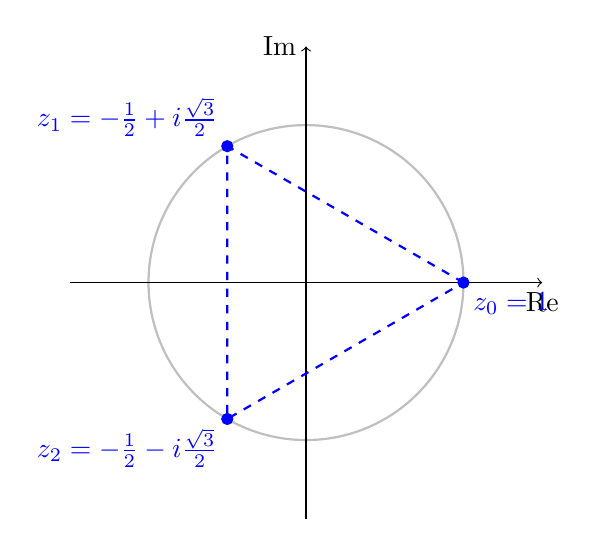
\begin{tikzpicture}[scale=2]
    % Cercle unité
    \draw[thick, gray!50] (0,0) circle(1);
    
    % Axes
    \draw[->] (-1.5,0) -- (1.5,0) node[below] {\( \text{Re} \)};
    \draw[->] (0,-1.5) -- (0,1.5) node[left] {\( \text{Im} \)};
    
    % Points sur le cercle
    \filldraw[blue] (1,0) circle(1pt) node[below right] {\( z_0 = 1 \)};
    \filldraw[blue] (-0.5,0.866) circle(1pt) node[above left] {\( z_1 = -\frac{1}{2} + i\frac{\sqrt{3}}{2} \)};
    \filldraw[blue] (-0.5,-0.866) circle(1pt) node[below left] {\( z_2 = -\frac{1}{2} - i\frac{\sqrt{3}}{2} \)};
    
    % Lignes de connexion
    \draw[thick, dashed, blue] (1,0) -- (-0.5,0.866) -- (-0.5,-0.866) -- cycle;
\end{tikzpicture}
\end{center}

Les racines cubiques de l'unité forment les sommets d'un triangle équilatéral inscrit dans le cercle unité dans le plan complexe.


\paragraph{\underline{\textbf{\textcolor{green}{Exemple 11: }}}}

Resoudre \( z^4 = 1, \) dans $\mathbb{C}$

Les \(4\) racines quatrièmes de l’unité sont données par la formule générale :
\[
z_k = e^{i\frac{2k\pi}{4}} = \cos\left(\frac{2k\pi}{4}\right) + i\sin\left(\frac{2k\pi}{4}\right), \quad k \in \{0, 1, 2, 3\}.
\]

\textbf{Calcul des racines :}
\begin{itemize}
    \item Pour \(k = 0\) : 
    \(
    z_0 = e^{i\frac{2\cdot 0\pi}{4}} = e^{i0} = 1.
    \)
    \item Pour \(k = 1\) : 
    \(
    z_1 = e^{i\frac{2\cdot 1\pi}{4}} = e^{i\frac{\pi}{2}} = \cos\left(\frac{\pi}{2}\right) + i\sin\left(\frac{\pi}{2}\right) = i.
    \)
    \item Pour \(k = 2\) : 
    \(
    z_2 = e^{i\frac{2\cdot 2\pi}{4}} = e^{i\pi} = \cos(\pi) + i\sin(\pi) = -1.
    \)
    \item Pour \(k = 3\) : 
    \(
    z_3 = e^{i\frac{2\cdot 3\pi}{4}} = e^{i\frac{3\pi}{2}} = \cos\left(\frac{3\pi}{2}\right) + i\sin\left(\frac{3\pi}{2}\right) = -i.
    \)
\end{itemize}

\textbf{Résultat :} Les \(4\) racines quatrièmes de l’unité sont :
\[
z_0 = 1, \quad z_1 = i, \quad z_2 = -1, \quad z_3 = -i.
\]

\textbf{Représentation graphique dans le plan complexe :}

\begin{center}
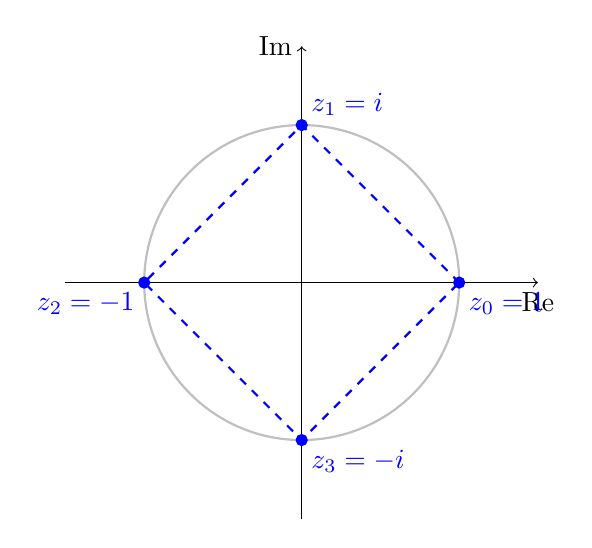
\begin{tikzpicture}[scale=2]
    % Cercle unité
    \draw[thick, gray!50] (0,0) circle(1);
    
    % Axes
    \draw[->] (-1.5,0) -- (1.5,0) node[below] {\( \text{Re} \)};
    \draw[->] (0,-1.5) -- (0,1.5) node[left] {\( \text{Im} \)};
    
    % Points sur le cercle
    \filldraw[blue] (1,0) circle(1pt) node[below right] {\( z_0 = 1 \)};
    \filldraw[blue] (0,1) circle(1pt) node[above right] {\( z_1 = i \)};
    \filldraw[blue] (-1,0) circle(1pt) node[below left] {\( z_2 = -1 \)};
    \filldraw[blue] (0,-1) circle(1pt) node[below right] {\( z_3 = -i \)};
    
    % Lignes de connexion
    \draw[thick, dashed, blue] (1,0) -- (0,1) -- (-1,0) -- (0,-1) -- cycle;
\end{tikzpicture}
\end{center}

Les racines quatrièmes de l'unité forment les sommets d'un carré inscrit dans le cercle unité dans le plan complexe.

\underline{\textbf{\textcolor{blue}{b.Racine nième d'un nombre complexe}}}\\
Soit $U \in \mathbb{C}$ et n un entier naturel différent de zéro.\\
L'équation $z^{n}=U$, $\theta=arg(z)$, a n solutions de la forme.\\
$z_{k}=\sqrt[n]{|U|}e^{i(\frac{\theta+2k\pi}{n})}$ avec $ 0\leq k \leq n-1 $.\\
\underline{\exemple}\\
Résoudre l'equation $z^{4}=\sqrt{2}+\sqrt{2}i$\\
$U=\sqrt{2}+\sqrt{2}i \Longrightarrow z_{k}=\sqrt[4]{|U|}e^{i(\frac{\theta+2k\pi)}{4}}$ avec 
$\theta=\frac{\pi}{4}$\\
\underline{\textbf{\textcolor{blue}{c. Propiétés}}}\\
Soit $z_{k}=\sqrt[n]{|U|}e^{i(\frac{\theta+2k\pi)}{n}}$\\
Les racines $z_{0}$ ; $z_{1}$ ; $z_{2}$ ; $z_{3}$ ; $z_{4}$ ; $z_{5}$ ; ... ; $z_{k-1}$ sont représentées dans le plan complexe par les points $M_{0}$ ; $M_{1}$ ; $M_{2}$ ; $M_{3}$ ; $M_{4}$ ; $M_{5}$ ; ... ; $M_{k-1}$ qui sont les sommets d’un polygone régulier inscrit dans le cercle de rayon $\sqrt[n]{|U|}$.\\
\underline{\textbf{\textcolor{blue}{d.Racinne carrée d'un nombre complexe}}}\\
Soit \( z \in \mathbb{C} \), un nombre complexe écrit sous la forme \( z = a + bi \) avec \( a, b \in \mathbb{R} \).  
Trouver les racines carrées de \( z \), c'est résoudre l'équation \( z = w^2  \), où \( w = x + yi \) est un nombre complexe, avec \( x, y \in \mathbb{R} \).  

En développant \( w^2 \), on obtient :  
\[
(x + yi)^2 = x^2 - y^2 + 2xyi = a + bi.
\]

Cela donne le système suivant :
\[
\begin{cases}
x^2 - y^2 = a, \\
2xy = b.
\end{cases}
\]

Par ailleurs, puisque \( z = w^2 \), on a \( |z| = |w^2| \). Comme \( |w^2| = |w|^2 \), il en résulte que :  
\[
x^2 + y^2 = \sqrt{a^2 + b^2}.
\]

Ainsi, on obtient un système de trois équations :  
\[
\begin{cases}
x^2 - y^2 = a, \\
2xy = b, \\
x^2 + y^2 = \sqrt{a^2 + b^2}.
\end{cases}
\]

Ce système peut être utilisé pour déterminer les valeurs de \( x \) et \( y \), et ainsi les deux racines carrées de \( z \) :
\[
w_1 = x + yi \quad \text{et} \quad w_2 = -x - yi.
\]

\paragraph{\underline{\textbf{\textcolor{blue}{Exemple :}}}}

Trouvons les racines carrées de \( z = 3 + 4i \).

\textbf{Étape 1 : Établir le système d'équations}  
Le nombre complexe \( z = 3 + 4i \) est écrit sous la forme \( z = a + bi \), avec \( a = 3 \) et \( b = 4 \).  

Le système à résoudre est :
\[
\begin{cases}
x^2 - y^2 = a, \\
2xy = b, \\
x^2 + y^2 = \sqrt{a^2 + b^2}.
\end{cases}
\]

Calculons \( \sqrt{a^2 + b^2} \) :
\[
\sqrt{a^2 + b^2} = \sqrt{3^2 + 4^2} = \sqrt{9 + 16} = \sqrt{25} = 5.
\]

Ainsi, le système devient :
\[
\begin{cases}
x^2 - y^2 = 3, \\
2xy = 4, \\
x^2 + y^2 = 5.
\end{cases}\implies
\begin{cases}
x^2 - y^2 = 3, \\
x^2 + y^2 = 5,\\
2xy = 4.
\end{cases}\implies
\begin{cases}
x^2 = 4, \\
y^2 = 1,\\
2xy = 4.
\end{cases}\implies
\begin{cases}
x = 2 \textbf{ ou } x = -2, \\
y = 1 \textbf{ ou } y = -1,\\
2xy = 4.
\end{cases}
\]
\textbf{Étape 2 : Résoudre le système}  
De \( x^2 + y^2 = 5 \) et \( x^2 - y^2 = 3 \), additionnons les deux équations :
\[
2x^2 = 8 \implies x^2 = 4 \implies x = \pm 2.
\]

Si \( x = 2 \), utilisons \( 2xy = 4 \) pour trouver \( y \) :
\[
2(2)y = 4 \implies y = 1.
\]

Si \( x = -2 \), alors \( 2(-2)y = 4 \) donne :
\[
y = -1.
\]

\textbf{Étape 3 : Les solutions}  
Les deux solutions sont :
\[
w_1 = x + yi = 2 + i, \quad w_2 = -x - yi = -2 - i.
\]

\textbf{Résultat final :}  
Les racines carrées de \( z = 3 + 4i \) sont :
\[
w_1 = 2 + i \quad \text{et} \quad w_2 = -2 - i.
\]

\textbf{Résoudre dans \( \mathbb{C} \) l’équation \( z^2 - (1 + i)z + i = 0 \).}

3. \textbf{Trouver \( \sqrt{\Delta} \) en utilisant la méthode \( z = w^2 \) :}  
On cherche \( \sqrt{\Delta} \), où \( \Delta = -2i \), en résolvant \( w^2 = -2i \).  
Posons \( w = x + yi \), avec \( x, y \in \mathbb{R} \). Alors :
\[
(x + yi)^2 = x^2 - y^2 + 2xyi = -2i.
\]

Cela donne le système suivant :
\[
\begin{cases}
x^2 - y^2 = 0, \\
2xy = -2.
\end{cases}
\]

\textbf{Résolution :}
- De \( x^2 - y^2 = 0 \), on a \( x^2 = y^2 \), donc \( y = \pm x \).
- Substituons \( y = x \) dans \( 2xy = -2 \) :
  \[
  2x(x) = -2 \implies 2x^2 = -2 \implies x^2 = 1 \implies x = \pm 1.
  \]
  Si \( x = 1 \), alors \( y = 1 \).  
  Si \( x = -1 \), alors \( y = -1 \).

\textbf{Les solutions pour \( w \) sont :}
\[
w_1 = 1 - i \quad \text{et} \quad w_2 = -1 + i.
\]

Ainsi, \( \sqrt{\Delta} = 1 - i \) ou \( \sqrt{\Delta} = -1 + i \).

4. \textbf{Appliquer la formule des solutions :}  
Les solutions de l’équation quadratique sont données par :
\[
z = \frac{-b \pm \sqrt{\Delta}}{2a}.
\]

- Pour \( \sqrt{\Delta} = 1 - i \) :
  \[
  z_1 = \frac{-(-1 - i) + (1 - i)}{2} = \frac{1 + i + 1 - i}{2} = \frac{2}{2} = 1.
  \]

- Pour \( \sqrt{\Delta} = -1 + i \) :
  \[
  z_2 = \frac{-(-1 - i) - (-1 + i)}{2} = \frac{1 + i - (-1 + i)}{2} = \frac{1 + i + 1 - i}{2} = \frac{2i}{2} = i.
  \]

\textbf{Résultat final :}  
Les solutions de \( z^2 - (1 + i)z + i = 0 \) sont :
\[
z_1 = 1 \quad \text{et} \quad z_2 = i.
\]
\subsection*{\underline{\textbf{\textcolor{red}{2.Résoudre une équation :}}}}
\underline{\textbf{\textcolor{green}{Exemple 11: }}}
Soit $(E)$ l’équation définie par $(E)$ : 
\[
z^3 - 3z^2 + (3 - i)z - 2(1 - i) = 0.
\]

\begin{enumerate}
    \item Montrer que $(E)$ admet une solution réelle à déterminer.

    \item Résoudre $(E)$.
\end{enumerate}
\underline{\textbf{\textcolor{red}{Solution}}}\\

\begin{enumerate}
    \item Soit $z = a$ la solution réelle de $(E)$.

    Donc,
    \[
    a^3 - 3a^2 + (3 - i)a - 2(1 - i) = 0
    \]
    \[
    \implies a^3 - 3a^2 + 3a - ai - 2 + 2i = 0
    \]
    \[
    \implies a^3 - 3a^2 + 3a - 2 + i(2 - a) = 0.
    \]

    Cela implique :
    \[
    \begin{cases}
    a^3 - 3a^2 + 3a - 2 = 0 \\
    2 - a = 0
    \end{cases}
    \]

    \[
    \implies
    \begin{cases}
    a^3 - 3a^2 + 3a - 2 = 0 \quad (1) \\
    a = 2 \quad (2)
    \end{cases}
    \]

    $a = 2$ vérifie aussi l’équation $(1)$, donc $2$ est la solution réelle cherchée.
\end{enumerate}
\begin{enumerate}
    \setcounter{enumi}{1}
    \item L’équation $(E)$ devient $(z - 2)(az^2 + bz + c) = 0$.  
    En procédant par exemple par la méthode de Hörner, on détermine les coefficients $a$, $b$ et $c$.

    On a : 
    \[
    (z - 2)(z^2 - z + 1 - i) = 0 \iff z = 2 \quad \text{ou} \quad z^2 - z + 1 - i = 0.
    \]

    Soit l’équation $z^2 - z + 1 - i = 0$, alors :
    \[
    \Delta = (1)^2 - 4(1)(1 - i) = 1 - 4 + 4i = -3 + 4i = (1 + 2i)^2.
    \]

    Donc :
    \[
    z_1 = \frac{1 - 1 - 2i}{2} = -i \quad \text{et} \quad z_2 = \frac{1 + 1 + 2i}{2} = 1 + i.
    \]

    D’où :
    \[
    S_C = \{2; -i; 1 + i\}.
    \]
\end{enumerate}

\[
\begin{array}{|c|c|c|c|c|}
\hline
 & 1 & 1 & 1 & 1  \\ 
\hline
-1 & \times & -1 & 0 & -1 \\ 
\hline
 & 1 & 0 & 1 & 0  \\
\hline
\end{array}
\]

\section*{\underline{\textbf{\textcolor{red}{IX.Interprétation géométrique des nombres complexes}}}}
\subsection*{\underline{\textbf{\textcolor{red}{Interprétation de $|\frac{d-c}{b-a}|$}}}}
Soit a,b,c et d des nombres complexes qui ont comme image A; B; C; D tel que $a \neq b$ et $c \neq d$\\
$|\frac{d-c}{b-a}|=\frac{CD}{AB}$\\
$arg(\frac{d-c}{b-a})=(\vec{AB},\vec{CD})$\\
\underline{\textbf{\textcolor{red}{Réel}}}\\
Si $\frac{d-c}{b-a} \in \mathbb{R}^{*}_{+}$ alors $\widehat{(\vec{AB},\vec{CD})}=0 [2\pi]$\\ 
Si $\frac{d-c}{b-a} \in \mathbb{R}^{*}_{-}$ alors $\widehat{(\vec{AB},\vec{CD})}=\pi [2\pi]$\\
\underline{\textbf{\textcolor{red}{imaginaire pur}}}\\
Si $\frac{d-c}{b-a} \in i\mathbb{R}^{*}_{+}$ alors $\widehat{(\vec{AB},\vec{CD})}=\frac{\pi}{2} [2\pi]$\\ 
Si $\frac{d-c}{b-a} \in i\mathbb{R}^{*}_{-}$ alors $\widehat{(\vec{AB},\vec{CD})}=-\frac{\pi}{2} [2\pi]$\\
\underline{\exemple}\\
Soit $Z=\frac{iz+2}{z+i}$ un nombre complexe\\
Détermine l'ensemble des points M tel que: $|Z'|=1$ puis $|Z'|=2$\\
\underline{\textbf{\textcolor{red}{Solution}}}\\
$|Z'|=|\frac{i(z-2i)}{z+i}|$\\
Soit $M(z)$ ; $A(2i)$ et $B(-i)$ alos on a:\\
$|Z'|=|\frac{i(z_{M}-z_{B})}{z_{M}-z_{A}}|=\frac{|i|\times|(z_{M}-z_{B})|}{|z_{M}-z_{A}|}=\left| \frac{MB}{MA}\right| $\\
Si $|Z'|=1$ alors $\frac{MA}{MB}=1 \Longrightarrow MA=MB$\\
L'ensemble des points $M$ tel que  $|Z'|=1$ est la médiatrice $[AB]$\\
++++++++++++++++++++++++++++++++++++++++++++++++
\section*{Configurations géométriques}

\begin{itemize}
    \item \textbf{Condition d'alignement} :  
    $A(a)$, $B(b)$ et $C(c)$ sont alignés si et seulement si $(b - a)(\overline{c} - \overline{a})$ est réel.

    \item \textbf{Condition d'orthogonalité} :  
    Les droites $(AB)$ et $(AC)$ sont orthogonales si et seulement si $(b - a)(\overline{c} - \overline{a})$ est imaginaire pur.

    \item \textbf{Condition de cocyclicité} :  
   % $A(a)$, $B(b)$, $C(c)$ et $D(d)$ sont alignés ou cocycliques si et seulement si :
    %\[
    %\frac{(d - a)(\overline{c} - \overline{b})}{(c - a)(\overline{d} - \overline{b})} \text{ est réel.}
    %\]
%ou \[
%\angle (\overrightarrow{CA}, \overrightarrow{CB}) = \angle (\overrightarrow{DA}, \overrightarrow{DB}) \mod \pi.
%\]
%ou
%\[
%\frac{\frac{c - b}{c - a}}{\frac{d - b}{d - a}} \text{ est réel.}
%\]

% Cercle
%\draw[thick] (0,0) circle(3);

% Points A, B, C, D
%\node[below left] at (-2.5,-1.5) {$A$};
%\node[below right] at (2.5,-1.5) {$B$};
%\node[above] at (0,2.7) {$C$};
%\node[right] at (2.5,1.5) {$D$};

% Sommets du cercle
%\coordinate (A) at (-2.5,-1.5);
%\coordinate (B) at (2.5,-1.5);
%\coordinate (C) at (0,2.7);
%\coordinate (D) at (2.5,1.5);

% Arcs et segments
%\draw[thick] (A) -- (C) -- (B);
%\draw[thick] (C) -- (D);
%\draw[thick] (A) -- (B);
%\draw[thick] (B) -- (D);

%\end{tikzpicture}

    \item \textbf{Triangle équilatéral} :  
    Les points $A(a)$, $B(b)$ et $C(c)$ forment un triangle équilatéral direct si, et seulement si :  
    \[
    a + j b + j^2 c = 0.
    \]

    \item \textbf{Barycentre} :  
    Si $G$ est le barycentre des points $M_k$ d’affixe $z_k$, affectés des coefficients $x_k$, alors l’affixe de $G$ est :
    \[
    \frac{1}{\sum_{k=1}^n x_k} \left( \sum_{k=1}^n x_k z_k \right).
    \]
\end{itemize}

\end{document}